\typeout{IJCAI--ECAI 26 Preprint}

\documentclass{article}
\pdfpagewidth=8.5in
\pdfpageheight=11in

\usepackage{ijcai26}
\usepackage{times}
\usepackage{url}
\usepackage{hyperref}
\usepackage[utf8]{inputenc}
\usepackage[small]{caption}
\usepackage{graphicx}
\usepackage{array}
\usepackage{amssymb}
\usepackage{amsmath}
\usepackage{float}
\usepackage{dblfloatfix}
\usepackage{booktabs}
\usepackage{tabularx}
\usepackage{placeins}
\usepackage[switch]{lineno}
\usepackage{tikz}
\usepackage{pgfplots}
\usetikzlibrary{arrows.meta,positioning,shapes.geometric}
\pgfplotsset{compat=1.18}

\hypersetup{
    colorlinks=true,
    linkcolor=blue,        
    citecolor=blue,        
    filecolor=magenta,     
    urlcolor=cyan,       
    pdftitle={Your Paper Title},
    pdfauthor={Your Name},
    pdfkeywords={keyword1, keyword2, keyword3},
    pdfpagemode=FullScreen,
}

% Comment out for a camera-ready version if the venue does not request line numbers.
\linenumbers
\urlstyle{same}

\pdfinfo{
/TemplateVersion (IJCAI.2026.0)
}

\title{A Decision-Making Framework for CI Failure Diagnosis with Incomplete Evidence and Uncertain Root Causes}

\author{
    Pradnyawant M. Gote
    \affiliations
    AI Engineer @ StatGlow
    \emails
    pradnyawantgote100@gmail.com
}

\begin{document}
\maketitle

\begin{abstract}
Continuous integration (CI) systems reveal where a workflow stopped, but the
failed stage alone rarely identifies why it failed. This paper asks whether a
diagnostic agent can decide which evidence to collect next instead of making a
one-shot root-cause prediction. We formulate CI diagnosis as a finite-horizon
Bayesian decision process over four operational categories: Code, Test,
Dependency, and CI/Config. A stage-conditioned prior is initialized from 309
mapped records in a 375-failure GitHub Actions dataset. The agent then selects
read-only diagnostic actions using expected Bayes-risk reduction per unit cost,
updates its belief from binary outcomes, and either reports a category or
refers the case for human review. In a deterministic simulation of 40 balanced
cases, the proposed policy produced 17 correct and one incorrect automatic
report, corresponding to 45.0\% coverage and 94.44\% selective accuracy. Its
configured total decision cost was 589.0, compared with 643.0 for
information-gain-per-cost, 603.5 for the lowest-cost policy, and 1020.0 for a
stage-MAP baseline. The stage baseline reported every case but made 22 errors.
However, the proposed policy referred all Test cases and eight of ten Code
cases, and its single error was reported with 0.9334 confidence. The study
therefore demonstrates an inspectable cost--risk trade-off inside a controlled
simulator; it does not establish production accuracy because action
likelihoods, outcomes, and costs are modeled rather than measured.
\end{abstract}

\section{Introduction}
\label{sec:introduction}

Continuous integration provides rapid feedback on whether software changes can
be built, tested, and delivered, but a failed workflow is an observation rather
than an explanation~\cite{Shahin2017Continuous}. Source-code defects, failing
tests, dependency changes, and workflow or environment faults can interrupt the
same pipeline stage. In a recent empirical study, Zheng et
al.~\cite{Zheng2026WorkflowFailures} manually examined 375 failed GitHub Actions
runs from 260 Java projects and reported a broad taxonomy of causes. Other
evidence shows that some build failures are unrelated to the triggering
patch~\cite{Huang2026UnrelatedFailures}. These findings make one-shot diagnosis
from the stage or latest commit a weak foundation for action.

Automated systems increasingly extract useful log evidence and generate
failure explanations. LogSage combines log processing, LLM-based diagnosis,
retrieval, and remediation~\cite{Xu2025LogSage}, while Auto-Diagnose presents
log-grounded integration-test summaries inside Google's review
workflow~\cite{Ziftci2026AutoDiagnose}. These systems address how evidence can
be interpreted. The complementary question studied here is how an agent should
choose the \emph{next} investigation when several causes remain plausible and
diagnostic checks have different costs.

We model that choice as sequential, decision-theoretic troubleshooting
~\cite{Heckerman1995Troubleshooting}. The agent maintains a belief over Code,
Test, Dependency, and CI/Config, predicts the possible outcomes of each
available read-only test, and greedily selects the action with the largest
expected reduction in reporting risk per unit cost. The belief is updated
after each outcome, and the episode ends with an automatic report only when a
confidence and loss gate is met; otherwise the evidence is referred to a
person. This design follows Bayesian experimental-design principles
~\cite{Rainforth2024ExperimentalDesign}, but it is a one-step policy rather
than an optimal multi-step planner.

The contribution is threefold. First, the study gives a transparent
probability-and-decision model for evidence acquisition, reporting, and
referral. Second, it evaluates four policies on the same balanced cases and
pre-generated outcome bank using coverage, conditional accuracy, probability
quality, diagnostic effort, and asymmetric decision cost. Third, it audits the
belief trajectories behind the observed high-confidence errors. The scope is
deliberately limited: historical records provide labels and stage context,
whereas diagnostic likelihoods, binary outcomes, and costs are declared or
simulated. The reported numbers describe this controlled model, not unseen
repositories or live incident response.

\section{Related Work}
\label{sec:related_work}

Empirical studies show that a failed run can have several explanations. Zheng
et al.~\cite{Zheng2026WorkflowFailures} provide the GitHub Actions taxonomy and
replication data used in this study. Huang et
al.~\cite{Huang2026UnrelatedFailures} examine failures unrelated to the current
patch, while Huang and Lin~\cite{Huang2026WorkflowReruns} study reruns whose
outcomes can change without repository modifications. Together, these studies
support separating the observed failure, the triggering change, and the
underlying cause.

Prior tools operate at finer granularity than the four-category belief used
here. BuildSheriff groups related CI test failures using change and failure
information~\cite{Zhang2022BuildSheriff}; UniLoc retrieves suspicious source
and build-script files from failure logs~\cite{Hassan2023UniLoc}; and LogChunks
provides 797 annotated Travis CI logs for evaluating failure-evidence
retrieval~\cite{Brandt2020LogChunks}. These methods could become evidence
producers for a future agent, whereas the present experiment assumes binary
outcomes and studies their selection order.

Recent work uses LLMs to summarize or resolve CI failures. Developer evaluation
of GitHub Actions explanations found encouraging results for simpler logs but
continued difficulty with complex scenarios
~\cite{ValenzuelaToledo2025GHAFailures}. LogSage evaluates an end-to-end
diagnosis and remediation pipeline~\cite{Xu2025LogSage}, and Auto-Diagnose
reports deployment evidence for integration-test assistance at
Google~\cite{Ziftci2026AutoDiagnose}. The current agent is narrower: it neither
parses raw logs nor changes code or runtime state. It chooses among authorized
investigations and records why a report or referral was made.

Decision-theoretic troubleshooting combines diagnostic probabilities with the
costs of observations and wrong decisions~\cite{Heckerman1995Troubleshooting}.
Belief states similarly summarize uncertainty in partially observable
decision processes~\cite{Kaelbling1998POMDP}. Lindley's expected information
measure~\cite{Lindley1956Information} and modern Bayesian experimental design
~\cite{Rainforth2024ExperimentalDesign} motivate choosing observations before
their outcomes are known. Our model applies these established ideas to a CI
simulation, but differs from general POMDP planning by using a greedy one-step
score and a fixed state space. Its novelty lies in the inspectable connection
among evidence value, asymmetric reporting loss, investigation cost, and
human referral, not in a new Bayesian inference rule.

\section{Agent Design}
\label{sec:agent_design}

The agent treats continuous integration (CI) failure diagnosis as a sequence
of decisions under uncertainty. It maintains competing explanations for a
failure, chooses a diagnostic action, and revises its belief after observing
the result. Investigation ends with either a root-cause report or referral
to a human reviewer. This formulation draws on decision-theoretic
troubleshooting and belief-state reasoning
under partial observability~\cite{Heckerman1995Troubleshooting,Kaelbling1998POMDP}.
The proposed policy
uses a one-step estimate of the reduction in reporting loss to choose the
next action as illustrated in~Figure~\ref{fig:agent-framework}.

\subsection{State representation and evidence intake}

The hidden state $s^\star$ denotes the failure category for the current
incident. The model uses

\begin{equation}
\mathcal{S}=\{\text{Code},\text{Test},\text{Dependency},\text{CI/Config}\}.
\label{eq:agent_states}
\end{equation}

These are operational categories inherited from the project's mapping of
historical failure labels. In particular, a failure assigned to
\textit{Test} need not originate in the test code itself. Each incident is
assigned one category, and diagnostic actions are assumed to leave that
category unchanged during an investigation. Simultaneous faults are outside
this representation.

The evidence-intake interface organizes the failed stage, logs, test output,
recent code or dependency changes, and CI environment context. In the
current notebook, the agent receives a case identifier and normalized stage
initially, followed by binary diagnostic outcomes. Parsing the raw artifacts
is therefore an interface requirement rather than an implemented log-analysis
capability. The identifier is used for tracking and does not affect inference.

The implemented normalizer uses seven labels: Build, Test, Setup / Dependency,
Quality / Analysis, Deploy / Publish, Ambiguous, and Unknown. These refine the
build--test--deploy overview in the architecture. Missing stage information
maps to Unknown, while unmatched descriptions map to Ambiguous. Let $z$ be
the normalized stage and $\mathcal{Z}$ this seven-label vocabulary.

\subsection{Historical initialization}

The source workbook comes from the replication package of Zheng
et al.~\cite{Zheng2026WorkflowFailures}. The project's mapping retains 309
of its 375 records and excludes 66 records outside the four modeled
categories. The retained counts for Code, Test, Dependency, and CI/Config
are 54, 120, 91, and 44, respectively. These counts describe the selected
source population rather than the prevalence of failures across all CI
systems.

Let $n_s$ denote the number of retained records in category $s$, and
$n_{s,z}$ the number with category $s$ and stage $z$. Laplace smoothing
gives

\begin{align}
\widehat{P}(s)
&=\frac{n_s+\alpha}{N+\alpha|\mathcal{S}|},
\label{eq:agent_prior}\\
\widehat{P}(z\mid s)
&=\frac{n_{s,z}+\beta}{n_s+\beta|\mathcal{Z}|},
\label{eq:agent_stage_likelihood}
\end{align}

where $N=309$ and $\alpha=\beta=1$. The initial belief incorporates the
observed stage once:

\begin{equation}
b_0(s)=
\frac{\widehat{P}(z\mid s)\widehat{P}(s)}
{\sum_{u\in\mathcal{S}}\widehat{P}(z\mid u)\widehat{P}(u)}.
\label{eq:agent_initial_belief}
\end{equation}

Smoothing keeps a category or stage combination from receiving zero
probability solely because it is absent from the finite source sample.


\begin{figure*}[!h]
    \centering
    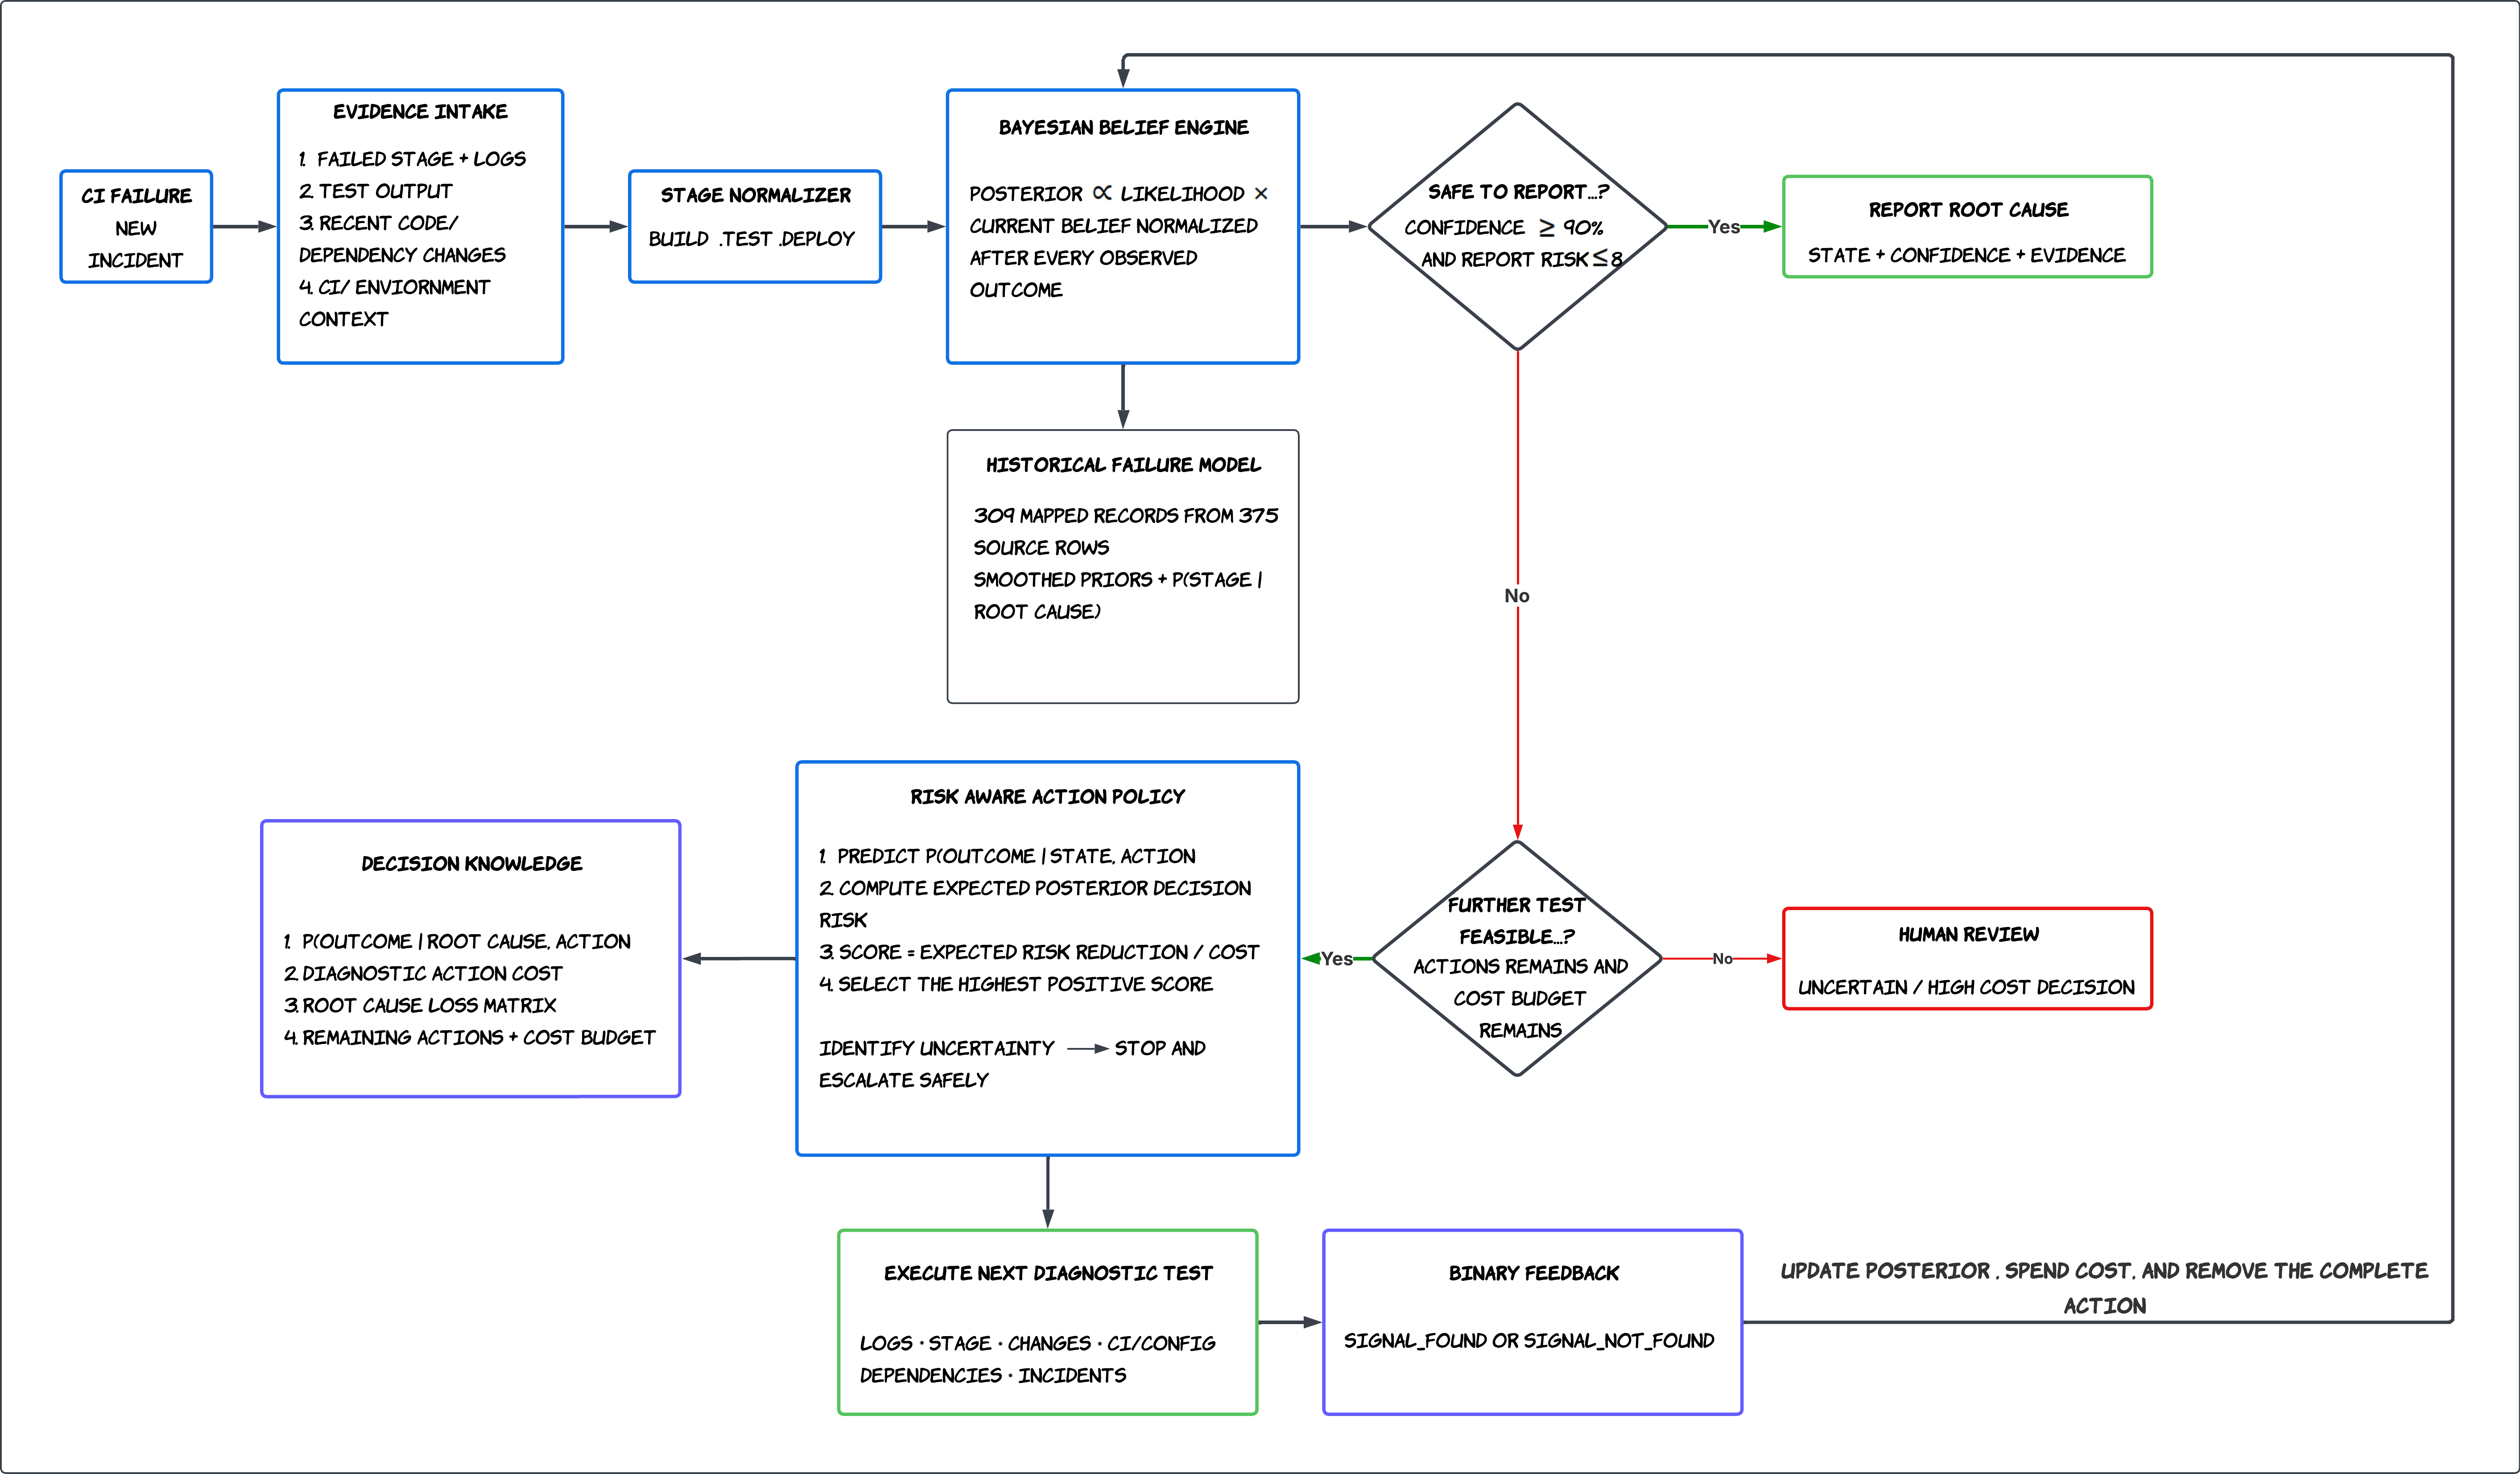
\includegraphics[width=1\linewidth]{figures/reasoning-framework.png}
    \caption{Conceptual architecture of agentic probability behavior and decision making.}
    \label{fig:agent-framework}
\end{figure*}


\subsection{Diagnostic actions and belief updates}

The action catalogue covers log inspection, failed-stage inspection,
comparison with the last successful run, recent changes, dependencies,
CI configuration, previous incidents, Docker images or caches, hosting,
and server or session state. Each action $a$ has a positive cost $c(a)$
and a set of eligible stages. Costs range from 1 to 2.5 relative effort
units; for example, dependency inspection costs 1 and CI configuration
inspection costs 2.5. These are declared modeling values rather than
measured durations or monetary costs.

An action returns $o\in\{0,1\}$, where 1 denotes
\texttt{SIGNAL\_FOUND} and 0 denotes \texttt{SIGNAL\_NOT\_FOUND}. Its
observation model is

\begin{equation}
\ell_a(o\mid s)=\theta_{s,a}^{\,o}(1-\theta_{s,a})^{1-o},
\qquad
\theta_{s,a}=P(o=1\mid s,a).
\label{eq:agent_observation_model}
\end{equation}

The diagnostic likelihoods $\theta_{s,a}$ are specified assumptions;
the historical workbook does not provide the action outcomes needed to
estimate them. A positive signal is evidence whose meaning depends on the
action, not a direct declaration of the true category.

At step $t$, the belief $b_t(s)$ represents the posterior probability of
category $s$ given the stage and outcomes observed so far. For a candidate
action, the predictive outcome probability and hypothetical posterior are

\begin{align}
q_t(o\mid a)
&=\sum_{s\in\mathcal{S}}b_t(s)\ell_a(o\mid s),
\label{eq:agent_predictive_outcome}\\
b_t^{a,o}(s)
&=\frac{b_t(s)\ell_a(o\mid s)}{q_t(o\mid a)}.
\label{eq:agent_posterior}
\end{align}

The posterior is defined for outcomes with $q_t(o\mid a)>0$; zero-probability
branches contribute nothing to expectations. After observing $o_t$ from
the selected action $a_t$, the agent sets $b_{t+1}=b_t^{a_t,o_t}$.

Using fixed action likelihoods assumes that outcomes are conditionally
independent given the hidden category and chosen actions. An additional
stage inspection must therefore provide a new clue, rather than count the
already observed stage a second time. Dependencies between signals from
overlapping logs or changes are a limitation of this model.

\subsection{Reporting loss and acceptance criteria}

Let $L(s,d)$ be the terminal loss of reporting category $d$ when the true
category is $s$. The configured loss matrix is

\begin{equation}
L=
\begin{pmatrix}
0 & 40 & 40 & 40\\
25 & 0 & 25 & 25\\
45 & 45 & 0 & 45\\
65 & 65 & 65 & 0
\end{pmatrix}.
\label{eq:agent_loss_matrix}
\end{equation}

Rows denote true categories and columns reported categories, both ordered
as Code, Test, Dependency, and CI/Config. A wrong report incurs the
true-category miss cost plus a fixed add-on of 5. The values express the
project's assumed consequences of misdiagnosis; they are not empirical
estimates of incident impact.

The expected loss of a report and the minimum reporting risk are

\begin{align}
r(d\mid b)&=\sum_{s\in\mathcal{S}}b(s)L(s,d),
\label{eq:agent_report_loss}\\
d_t^{\mathrm{risk}}&\in\arg\min_{d\in\mathcal{S}}r(d\mid b_t),
\qquad
R(b_t)=r(d_t^{\mathrm{risk}}\mid b_t).
\label{eq:agent_bayes_risk}
\end{align}

Here $R$ concerns root-cause reports only; it does not include human review
as a competing report. Define the maximum a posteriori (MAP) category as
$d_t^{\mathrm{MAP}}\in\arg\max_s b_t(s)$. Automatic reporting requires

\begin{equation}
\begin{aligned}
d_t^{\mathrm{MAP}}&=d_t^{\mathrm{risk}},\\
b_t(d_t^{\mathrm{MAP}})&\geq 0.90,\\
R(b_t)&\leq 8.
\end{aligned}
\label{eq:agent_reporting_gate}
\end{equation}

The risk threshold is expressed in the declared loss units, rather than as
a percentage. With this particular matrix, 90\% confidence already implies
agreement between the MAP and minimum-risk categories and a reporting loss
of at most $65(1-0.90)=6.5$. The other two checks are consequently redundant
at the current settings, although they remain explicit configuration
checks. The risk model still affects action selection at lower confidence.

\subsection{Selecting the next diagnostic action}

Let $\mathcal{U}_t$ be the unused actions and $B_t$ the remaining diagnostic
budget. After $t$ executed actions, the feasible set is

\begin{equation}
\mathcal{F}_t=
\left\{a\in\mathcal{U}_t:
a\text{ is eligible for }z,\ c(a)\leq B_t,\ t<8\right\},
\label{eq:agent_feasible_actions}
\end{equation}

with $B_0=11$. If reporting is not yet permitted, the agent evaluates how
each feasible action could change the best subsequent report:

\begin{align}
\overline{R}_t(a)
&=\sum_{o\in\{0,1\}}q_t(o\mid a)R(b_t^{a,o}),
\label{eq:agent_expected_posterior_risk}\\
\Delta R_t(a)&=R(b_t)-\overline{R}_t(a),
\label{eq:agent_risk_reduction}\\
V_t(a)&=\frac{\Delta R_t(a)}{c(a)}.
\label{eq:agent_action_score}
\end{align}

The minimum-risk report is recomputed separately for each hypothetical
outcome. This allows an action to be valuable because it could change the
reporting decision, even if it does not produce the largest reduction in
overall uncertainty.

Following the architecture, the design selects

\begin{equation}
a_t\in\arg\max_{a\in\mathcal{F}_t}V_t(a)
\quad\text{only if}\quad
\max_{a\in\mathcal{F}_t}V_t(a)>0.
\label{eq:agent_selected_action}
\end{equation}

Ties are resolved by larger expected risk reduction, then lower cost, then
action name. The positive-score condition is an explicit design
requirement: the current notebook ranks candidates but does not yet reject
an action whose score is zero. If the feasible set is empty or no positive
score remains, the design refers the incident for human review.

This is a greedy, one-step policy. It does not optimize complete sequences
of tests or guarantee the minimum total investigation cost. In particular,
a positive risk reduction does not by itself establish that the improvement
outweighs the action's cost under a common utility scale.

For comparison, the EIG-per-cost policy uses expected information gain:

\begin{equation}
I_t(a)=H(b_t)-\sum_{o\in\{0,1\}}q_t(o\mid a)H(b_t^{a,o}),
\label{eq:agent_eig_baseline}
\end{equation}

where $H(b)=-\sum_s b(s)\log_2 b(s)$, with $0\log_2 0=0$. That policy
ranks actions by $I_t(a)/c(a)$; the proposed policy ranks them by
Equation~\eqref{eq:agent_action_score}, which accounts for the specified
consequences of reporting errors.

\subsection{Execution, escalation, and audit trail}

After executing $a_t$ and updating the posterior, the agent updates its
resources:

\begin{equation}
B_{t+1}=B_t-c(a_t),
\qquad
\mathcal{U}_{t+1}=\mathcal{U}_t\setminus\{a_t\}.
\label{eq:agent_resource_update}
\end{equation}

It then checks the reporting conditions again, including after the last
permitted action. An accepted report contains the selected category,
posterior confidence, and supporting diagnostic outcomes. Otherwise,
exhaustion of the action count, affordable eligible actions, or positive
scores leads to human review with the evidence collected so far.

The configured terminal cost of referral is 12 units. For assessment, this
cost or the loss of an automatic report is added to the diagnostic costs
already incurred. Human review is an explicit terminal outcome; the model
does not simulate the reviewer's eventual diagnosis.

An audit record associates each action with its outcome, selection score,
belief update, cumulative cost, and stopping decision. In the current
prototype, diagnostic feedback is simulated using a perturbed likelihood
matrix. Moreover, the 40 evaluation cases are sampled from the same mapped
pool used to estimate the priors and stage likelihoods. Hiding their labels
during an episode therefore does not constitute an independent holdout
evaluation. Posterior confidence remains conditional on the assumed model,
and the 90\% threshold does not establish 90\% empirical accuracy.


% Requires \usepackage{amsmath,amssymb} in the document preamble.
% All citation keys are compatible with the earlier paper bibliography.
% Standalone bibliography: ci_probability_model_references.bib.
% Editorial note: the earlier Agent Design section contains overlapping
% equations. In the assembled paper, keep detailed derivations here and
% cross-reference them from the architectural description.

\section{Probability Model and Decision Rule}
\label{sec:probability_model_decision_rule}

The probability model represents the agent's uncertainty about a CI
failure, while the decision rule determines what to do with that uncertainty.
The agent maintains a distribution over possible failure categories and
updates it as diagnostic evidence becomes available. This use of a belief
state follows the treatment of partially observable decision
problems~\cite{Kaelbling1998POMDP}. In this project, the hidden category remains fixed
during an investigation; diagnostic actions gather information without
repairing the underlying fault.

\subsection{Prior belief and initial evidence}

Let $s^\star$ denote the unknown category, with
$\mathcal{S}=\{\text{Code},\text{Test},\text{Dependency},\text{CI/Config}\}$.
The four categories follow the project's mapping of historical labels.
They provide one operational label per incident rather than a model of
simultaneous faults. Let $E_t$ contain the normalized failed stage $z$ and
the $t$ action--outcome pairs observed so far. The belief is
\begin{equation}
b_t(s)=P(s^\star=s\mid E_t),
\qquad b_t(s)\geq 0,
\qquad \sum_{s\in\mathcal{S}}b_t(s)=1.
\label{eq:prob_belief}
\end{equation}

The historical records originate from the replication package of Zheng
et al.~\cite{Zheng2026WorkflowFailures}. The project retains 309 of the
375 records, with category counts $(54,120,91,44)$ in the order given above.
The remaining 66 records are outside the selected mapping. Let $n_s$ be a
category count and $n_{s,z}$ its count at stage $z$. The smoothed prior and
stage likelihood are
\begin{align}
\widehat{P}(s)
&=\frac{n_s+\alpha}{N+\alpha|\mathcal{S}|},
\label{eq:prob_prior}\\
\widehat{P}(z\mid s)
&=\frac{n_{s,z}+\beta}{n_s+\beta|\mathcal{Z}|},
\label{eq:prob_stage}
\end{align}
where $N=309$, $\alpha=\beta=1$, and $|\mathcal{Z}|=7$. The implemented
stage vocabulary includes Build, Test, Setup / Dependency, Quality /
Analysis, Deploy / Publish, Ambiguous, and Unknown. The prior vector is
therefore $(55,121,92,45)/313$. These probabilities describe the mapped
source records, not the prevalence of failures across all CI environments.

The failed stage supplies the initial evidence:
\begin{equation}
b_0(s)=
\frac{\widehat{P}(z\mid s)\widehat{P}(s)}
{\sum_{u\in\mathcal{S}}\widehat{P}(z\mid u)\widehat{P}(u)}.
\label{eq:prob_initial_posterior}
\end{equation}
This separates the prior frequency of a category from the evidence supplied
by the current failure. The stage is incorporated once at initialization.

\subsection{Observation model and posterior updates}

Each diagnostic action $a$ returns a binary outcome $o\in\{0,1\}$,
corresponding to \texttt{SIGNAL\_NOT\_FOUND} and \texttt{SIGNAL\_FOUND},
respectively. Define the action likelihoods as
\begin{equation}
\ell_a(1\mid s)=\theta_{s,a},
\qquad
\ell_a(0\mid s)=1-\theta_{s,a}.
\label{eq:prob_binary_likelihood}
\end{equation}
Here $\theta_{s,a}$ is the probability of finding the action-specific signal
when the true category is $s$. These parameters are declared assumptions,
because the historical workbook does not contain the diagnostic outcomes
needed to estimate them. A signal is evidence about a category, rather than
an observation of the category itself.

The model assumes that a new outcome depends on the hidden category and
selected action, with no additional dependence on previously observed
evidence. Under this assumption, the predictive outcome probability and
posterior are
\begin{align}
q_t(o\mid a)
&=\sum_{s\in\mathcal{S}}b_t(s)\ell_a(o\mid s),
\label{eq:prob_predictive}\\
b_t^{a,o}(s)
&=\frac{b_t(s)\ell_a(o\mid s)}{q_t(o\mid a)}.
\label{eq:prob_update}
\end{align}
The posterior is evaluated for outcomes with positive predictive
probability. After observing $o_t$ from the executed action $a_t$, the agent
sets $b_{t+1}=b_t^{a_t,o_t}$. Both positive and negative results can change
the diagnosis. For example, an absent dependency signal reduces belief in
a dependency failure when that absence is unlikely under the dependency
hypothesis. Correlated signals or repeated use of the same evidence can
produce excessive confidence under the independence assumption.

\subsection{Expected reporting loss}

The most probable category is not necessarily the preferred report when
different errors carry different consequences. Following a decision-theoretic
approach to troubleshooting~\cite{Heckerman1995Troubleshooting}, let $L(s,d)$
be the loss of reporting category $d$ when the true category is $s$. The
configured loss can be written compactly as
\begin{equation}
L(s,d)=w_s\,\mathbf{1}\{s\neq d\},
\qquad \boldsymbol{w}=(40,25,45,65).
\label{eq:prob_loss}
\end{equation}
The weights follow the category order given above. Each weight includes
the category-specific miss cost and the fixed
wrong-report add-on of 5. A correct report has zero terminal loss. The
weights are project assumptions expressed in relative loss units.

The expected loss of report $d$ and the minimum reporting risk are
\begin{align}
r(d\mid b)&=\sum_{s\in\mathcal{S}}b(s)L(s,d),
\label{eq:prob_expected_loss}\\
R(b)&=\min_{d\in\mathcal{S}}r(d\mid b).
\label{eq:prob_bayes_risk}
\end{align}
For this loss structure, the minimum-risk report has a useful closed form:
\begin{equation}
\begin{aligned}
d_t^{\mathrm{risk}}
&\in\arg\max_{d\in\mathcal{S}}w_d b_t(d),\\
R(b_t)
&=\sum_{s\in\mathcal{S}}w_s b_t(s)
  -\max_{d\in\mathcal{S}}w_d b_t(d).
\end{aligned}
\label{eq:prob_weighted_decision}
\end{equation}
Thus a category with a larger miss cost can become the preferred report
before it becomes the most probable category. Ties between reporting
categories follow the fixed category order. Human review is excluded from
$R(b)$, which measures the loss of the best root-cause report only.

\subsection{Selecting evidence by expected risk reduction}

Before executing an action, the agent considers both possible outcomes
and the report it would prefer after each one. This is an expected-utility
calculation over hypothetical observations, as used in Bayesian
experimental design~\cite{Rainforth2024ExperimentalDesign}. For an action
with positive diagnostic cost $c(a)$, define
\begin{align}
\overline{R}_t(a)
&=\sum_{o\in\{0,1\}}q_t(o\mid a)R(b_t^{a,o}),
\label{eq:prob_expected_future_risk}\\
\Delta R_t(a)&=R(b_t)-\overline{R}_t(a),
\label{eq:prob_risk_reduction}\\
V_t(a)&=\frac{\Delta R_t(a)}{c(a)}.
\label{eq:prob_score}
\end{align}
Zero-probability outcomes contribute zero to the expectation. The reporting
decision is optimized separately within each outcome branch. Under the
specified probability model, $\Delta R_t(a)$ is nonnegative because
additional evidence can be ignored when choosing a report. However, an
individual observed outcome can increase reporting risk even when the
expected reduction is positive.

The score measures expected reduction in reporting loss per unit of
diagnostic effort. The EIG-per-cost comparison instead measures expected
entropy reduction per unit cost. The proposed score is a one-step
heuristic: it does not optimize complete action sequences or directly
compare every test with the cost of immediate human review. A positive
score also does not establish a positive net benefit after subtracting
test cost on a common utility scale.

\subsection{Reporting, further testing, and human review}

\vskip .1 in

Define $d_t^{\mathrm{MAP}}\in\arg\max_s b_t(s)$. The reporting indicator is
\begin{equation}
G_t=\mathbf{1}\!\left\{
d_t^{\mathrm{MAP}}=d_t^{\mathrm{risk}},\;
b_t(d_t^{\mathrm{MAP}})\geq 0.90,\;
R(b_t)\leq 8
\right\}.
\label{eq:prob_report_gate}
\end{equation}
The three requirements are conjunctive. The risk cap is measured in loss
units, not percent. With the configured weights, 90\% confidence already
implies MAP--minimum-risk agreement and report risk no greater than
$65(1-0.90)=6.5$. The agreement and risk-cap checks therefore provide no
additional filtering at these settings, although the asymmetric loss
continues to influence action selection at lower confidence.

Let $\mathcal{U}_t$ contain unused actions and $B_t$ be the remaining
diagnostic budget. After $t$ tests, the feasible and positive-score sets are
\begin{align}
\mathcal{F}_t
&=\{a\in\mathcal{U}_t:
a\text{ is eligible for }z,\ c(a)\leq B_t,\ t<8\},
\label{eq:prob_feasible}\\
\mathcal{F}_t^{+}
&=\{a\in\mathcal{F}_t:V_t(a)>0\},
\label{eq:prob_positive}
\end{align}
where $B_0=11$. When $\mathcal{F}_t^+$ is nonempty, select
$a_t^\star\in\arg\max_{a\in\mathcal{F}_t^+}V_t(a)$, breaking ties by
larger $\Delta R_t(a)$, lower cost, and then action name. For the decision
state $x_t=(b_t,z,\mathcal{U}_t,B_t,t)$, the architecture specifies
\begin{equation}
\pi(x_t)=
\begin{cases}
\mathrm{REPORT}(d_t^{\mathrm{risk}}), & G_t=1,\\
\mathrm{TEST}(a_t^\star), & G_t=0\text{ and }\mathcal{F}_t^+\neq\varnothing,\\
\mathrm{HUMAN\_REVIEW}, & \text{otherwise}.
\end{cases}
\label{eq:prob_policy}
\end{equation}
Following a test, the posterior is updated, its cost is deducted from
$B_t$, and the action is removed from $\mathcal{U}_t$. The reporting
condition is checked again, including after the eighth permitted test.
The positive-score restriction in this rule follows the diagram; the
inspected notebook ranks feasible actions but does not yet enforce that
restriction. Its existing evaluation therefore does not establish the
behavior of this additional stopping condition.

For an investigation ending after $T$ tests, the recorded total cost is
\begin{equation}
\resizebox{0.88\columnwidth}{!}{$\displaystyle
C_{\mathrm{episode}}=
\sum_{t=0}^{T-1}c(a_t)+
\begin{cases}
L(s^\star,d_T), & \text{if a category is reported},\\
12, & \text{if the case is referred for human review}.
\end{cases}
$}
\label{eq:prob_episode_cost}
\end{equation}https://www.overleaf.com/project/6aaad92441620dd50633edb9/download/zip

The true category is needed only to score a completed automatic report;
it is not revealed during the diagnostic episode. Nevertheless, the
prototype estimates its prior and stage likelihoods from the same mapped
pool from which its 40 evaluation cases are sampled, so those cases do not
constitute an independent holdout. Posterior confidence is conditional on
the model and its assumed likelihoods; a 90\% reporting threshold does not
by itself demonstrate 90\% empirical accuracy.

\begin{table*}[!b]
\renewcommand{\arraystretch}{1.2}
\centering
\caption{Terminal outcomes on the 40 balanced cases. Selective accuracy is
conditioned on automatic reports; OCA is the correct-automatic fraction of all
cases.}
\label{tab:decision_results}
\footnotesize
\begin{tabular*}{\textwidth}{@{\extracolsep{\fill}}lrrrrrrr@{}}
\toprule
Policy & Auto. & Correct & Wrong & Review & Coverage (\%) &
Sel. acc. (\%) & OCA (\%) \\
\midrule
Risk reduction/cost & 18 & 17 & 1  & 22 & 45.0  & 94.44 & 42.5 \\
EIG/cost            & 18 & 16 & 2  & 22 & 45.0  & 88.89 & 40.0 \\
Lowest cost         & 15 & 15 & 0  & 25 & 37.5  & 100.00 & 37.5 \\
Stage-MAP           & 40 & 18 & 22 & 0  & 100.0 & 45.00 & 45.0 \\
\bottomrule
\end{tabular*}
\end{table*}

\begin{table*}[!b]
\renewcommand{\arraystretch}{1.2}
\centering
\caption{Effort, configured total decision cost, and probability quality.}
\label{tab:quality_results}
\footnotesize
\begin{tabular*}{\textwidth}{@{\extracolsep{\fill}}lrrrrrr@{}}
\toprule
Policy & Mean actions & Mean diag. cost & Total cost &
Macro $F_1$ & Brier & ECE \\
\midrule
Risk reduction/cost & 4.325 & 6.5000 & 589.0  & 0.4958 & 0.2673 & 0.0387 \\
EIG/cost            & 4.575 & 6.8500 & 643.0  & 0.4703 & 0.3024 & 0.0863 \\
Lowest cost         & 5.200 & 7.5875 & 603.5  & 0.4722 & 0.2357 & 0.0668 \\
Stage-MAP           & 0.000 & 0.0000 & 1020.0 & 0.3824 & 0.6682 & 0.1222 \\
\bottomrule
\end{tabular*}
\end{table*}


% Requires \usepackage{amsmath,amssymb,url} in the document preamble.
% Citation keys are compatible with the preceding paper sections.
% Standalone bibliography: ci_test_method_references.bib.
% This section describes the executed notebook evaluation, not a live-CI test.

\section{Test Method}
\label{sec:test_method}

The experiment tests decision behavior under controlled model mismatch rather
than replaying raw logs or executing commands against live pipelines.
Table~\ref{tab:test_configuration} summarizes the complete configuration.

\begin{table}[!h]
\renewcommand{\arraystretch}{1.2}
\centering
\caption{Configuration of the deterministic evaluation.}
\label{tab:test_configuration}
\footnotesize
\begin{tabularx}{\columnwidth}{@{}lX@{}}
\toprule
Item & Setting \\
\midrule
Source & 375 GitHub Actions failures from 260 projects
~\cite{Zheng2026WorkflowFailures} \\
Mapped pool & 309 records: 54 Code, 120 Test, 91 Dependency, 44 CI/Config \\
Cases & 40 balanced cases (10 per state), sampled without replacement \\
Visible input & Case identifier and normalized failed stage; label hidden
during the episode \\
Policies & Risk reduction/cost, EIG/cost, lowest cost, and stage-MAP \\
Report gate & MAP equals minimum-risk label, confidence $\geq0.90$, risk
$\leq8$ \\
Resources & At most 8 actions, budget 11, review cost 12 \\
Outcome seeds & Likelihood perturbation: 20260826; outcome bank: 20260827 \\
\bottomrule
\end{tabularx}
\end{table}

\subsection{Cases, outcomes, and paired comparison}

The 40 labels are hidden from the policy but remain in the same 309-record pool
used to estimate priors and stage likelihoods. The evaluation is therefore
in-sample with hidden episode labels, not repository-disjoint validation. Since
the source records do not contain action outcomes, the harness perturbs the
agent likelihoods and pre-generates a shared outcome bank:
\begin{align}
\widetilde\theta_{s,a}
  &=\operatorname{clip}_{[0.02,0.98]}
    \!\left(0.82\theta_{s,a}+0.09+\varepsilon_{s,a}\right),
  \label{eq:simulator_probability}\\
\varepsilon_{s,a}
  &\sim\mathcal N(0,0.045^2),\qquad
O_{i,a}\sim\operatorname{Bernoulli}
  (\widetilde\theta_{y_i,a}).
  \label{eq:simulator_outcome}
\end{align}
Every policy receives the same outcome for the same case--action pair. This
paired design isolates policy choices within the fixed run, but it does not
replace repeated simulations or observed investigation traces.

The three sequential policies use identical actions, likelihoods, gates, and
budgets. Risk/cost ranks actions by Equation~\eqref{eq:prob_score};
EIG/cost ranks them by expected entropy reduction per cost; lowest cost chooses
the cheapest eligible test; and stage-MAP immediately reports the largest
component of $b_0$. The current implementation does not enforce the formal
positive-score guard.

\subsection{Measures and checks}

Let $A_i^\pi$ indicate an automatic report and
$K_i^\pi=\mathbf1\{\widehat y_i^\pi=y_i\}$. For $n=40$,
\begin{align}
\operatorname{Cov}_\pi
  &=\frac{1}{n}\sum_i A_i^\pi,
  \label{eq:coverage}\\
\operatorname{SelAcc}_\pi
  &=\frac{\sum_i A_i^\pi K_i^\pi}{\sum_i A_i^\pi},
  \label{eq:selective_accuracy}\\
\operatorname{OCA}_\pi
  &=\frac{1}{n}\sum_i A_i^\pi K_i^\pi.
  \label{eq:overall_correct_auto}
\end{align}
Selective accuracy is reported with coverage because abstention can improve
conditional accuracy by accepting fewer cases~\cite{Geifman2017Selective}.
Review rate is $1-\operatorname{Cov}_\pi$. Macro precision, recall, and $F_1$
are computed over the four states, with referrals counted as false negatives
for their true state.

The per-case total cost is
\begin{equation}
T_i^\pi=
\sum_{a\in\mathcal T_i^\pi}c(a)
+\mathbf1_{\mathrm{report}}L(y_i,\widehat y_i^\pi)
+12\,\mathbf1_{\mathrm{review}}.
\label{eq:test_total_cost}
\end{equation}
Probability quality is measured with the multiclass Brier score
~\cite{Brier1950Verification} and ten-bin ECE
~\cite{Guo2017Calibration}:
\begin{align}
\operatorname{BS}_\pi
  &=\frac{1}{n}\sum_i\sum_{s\in\mathcal S}
    \left(p_{is}^\pi-\mathbf1\{y_i=s\}\right)^2,
  \label{eq:brier}\\
\operatorname{ECE}_\pi
  &=\sum_{m=1}^{10}\frac{|\mathcal B_m|}{n}
    \left|\operatorname{acc}(\mathcal B_m)
    -\operatorname{conf}(\mathcal B_m)\right|.
  \label{eq:ece}
\end{align}
With only 40 cases, ECE is descriptive rather than evidence that the reporting
threshold is calibrated. Fresh-kernel checks verified normalized
probabilities, non-repeated actions, stage filtering, common outcome reuse,
budget accounting, and terminal report-or-review behavior. The run generated
160 terminal records and 564 action records.

\section{Results}
\label{sec:results}

Table~\ref{tab:decision_results} reports the central safety--coverage trade-off.
Risk reduction/cost automatically reported 18 cases: 17 correctly and one
incorrectly. Its 45.0\% coverage therefore corresponded to 94.44\% selective
accuracy. EIG/cost reached the same coverage but made two errors. Lowest cost
made no wrong automatic report, but referred 25 of 40 cases. Stage-MAP covered
every case while making 22 wrong reports.



The cost and probability measures do not identify one universally best policy as mentioned in Table~\ref{tab:quality_results}. Risk reduction/cost used 4.325 actions and
6.50 diagnostic-cost units per case. Its total decision cost was 589.0, which
was 8.4\% below EIG/cost, 2.4\% below lowest cost, and 42.3\% below stage-MAP.
It also had the largest macro-$F_1$ (0.4958) and smallest ECE (0.0387).
Lowest cost had the smallest Brier score (0.2357) and perfect selective
accuracy, but only 37.5\% coverage. These cost values are conditional on the
declared error, action, and referral costs; they are not time or money.



Coverage was uneven across states. The proposed policy correctly reported 2 of
10 Code, 0 of 10 Test, 9 of 10 Dependency, and 6 of 10 CI/Config cases. It
referred the remaining 8 Code, 10 Test, 1 Dependency, and 3 CI/Config cases,
and mislabeled one CI/Config case as Dependency. Thus, the aggregate selective
accuracy reflects strong Dependency and CI/Config performance combined with
substantial referral, not uniformly reliable diagnosis.

All unit and invariance checks passed in a fresh execution. This supports
internal reproducibility of the saved run, but not generalization: one balanced
sample, one outcome bank, and the same mapped pool for initialization and
sampling provide no confidence interval or independent repository test.

\section{Failure Analysis}
\label{sec:failure_analysis}

Incorrect reports and referrals have different meanings. A wrong automatic
report exposes the user to a false diagnosis; referral avoids forced guessing
but consumes human capacity. Across the sequential policies, three automatic
decisions were wrong, corresponding to two unique cases as mentioned in Table~\ref{tab:sequential_errors}. Lowest cost had no wrong report at 37.5\%
coverage, whereas stage-MAP bypassed the gate and made 22 errors.

\begin{table*}[!h]
\renewcommand{\arraystretch}{1.2}
\centering
\caption{All incorrect automatic reports made by the sequential policies.}
\label{tab:sequential_errors}
\footnotesize
\begin{tabular*}{\textwidth}{@{\extracolsep{\fill}}llllrr@{}}
\toprule
Policy & Case & Stage & True $\rightarrow$ report & Confidence & Total cost \\
\midrule
Risk/cost & CI-007 & Quality/Analysis &
CI/Config $\rightarrow$ Dependency & 0.9334 & 68.5 \\
EIG/cost & CI-007 & Quality/Analysis &
CI/Config $\rightarrow$ Dependency & 0.9334 & 68.5 \\
EIG/cost & CI-012 & Build &
Code $\rightarrow$ CI/Config & 0.9052 & 48.5 \\
\bottomrule
\end{tabular*}
\end{table*}


\begin{figure*}[!b]
\centering
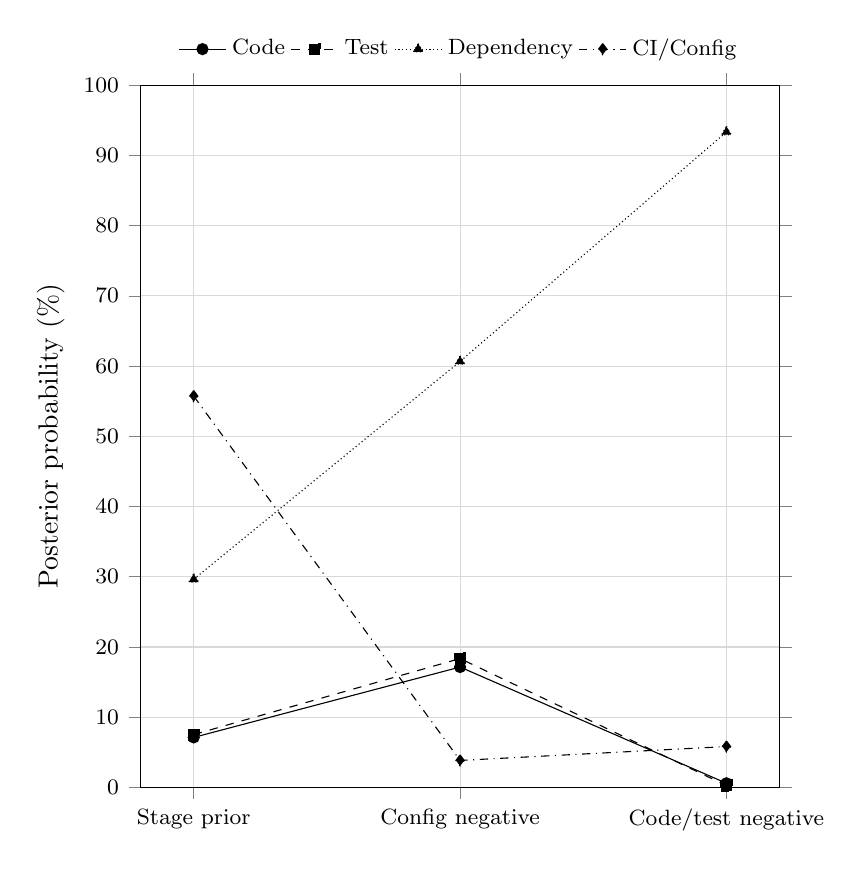
\begin{tikzpicture}
\begin{axis}[
    width=0.8\textwidth,
    height=10.5cm,
    ymin=0, ymax=100,
    ylabel={Posterior probability (\%)},
    symbolic x coords={Stage prior,Config negative,Code/test negative},
    xtick=data,
    x tick label style={font=\footnotesize, align=center},
    y tick label style={font=\footnotesize},
    legend style={at={(0.5,1.02)},anchor=south,legend columns=4,
        draw=none,font=\footnotesize},
    grid=major,
    major grid style={black!15},
    axis line style={black},
    tick align=outside
]
\addplot[black, solid, mark=*] coordinates {
    (Stage prior,7.12) (Config negative,17.14) (Code/test negative,0.59)};
\addlegendentry{Code}
\addplot[black, dashed, mark=square*] coordinates {
    (Stage prior,7.52) (Config negative,18.35) (Code/test negative,0.26)};
\addlegendentry{Test}
\addplot[black, densely dotted, mark=triangle*] coordinates {
    (Stage prior,29.64) (Config negative,60.66) (Code/test negative,93.34)};
\addlegendentry{Dependency}
\addplot[black, dashdotted, mark=diamond*] coordinates {
    (Stage prior,55.72) (Config negative,3.84) (Code/test negative,5.82)};
\addlegendentry{CI/Config}
\end{axis}
\end{tikzpicture}
\caption{Posterior trajectory for \texttt{CI-007}. }
\label{fig:ci007_trace}
\end{figure*}

\subsection{High-confidence errors}

The proposed policy's only error, \texttt{CI-007}, followed two negative
signals. For a negative outcome from action $a$, posterior odds change by
\begin{equation}
\frac{b_{t+1}(s_i)/b_{t+1}(s_j)}
     {b_t(s_i)/b_t(s_j)}
=\frac{1-\theta_{s_i,a}}{1-\theta_{s_j,a}}.
\label{eq:negative_bayes_factor}
\end{equation}
The missing CI/configuration signal had likelihood 0.831 under Dependency but
only 0.028 under the true CI/Config state, a Bayes factor of 29.68 in favor of
Dependency. The next negative code/test-change signal removed most remaining
Code and Test mass. As Figure~\ref{fig:ci007_trace} shows, the resulting
Dependency posterior reached 93.34\% and passed both gates. The error therefore
reflects likelihood misspecification, not a failure to apply Bayes' rule.


\texttt{CI-012}, observed only under EIG/cost, contained conflicting signals.
A positive code/test-change result initially favored Code; later positive
CI/environment evidence and two negative checks shifted the posterior to
90.52\% CI/Config. A fixed 0.90 gate cannot prevent error when the observation
model itself is overconfident. Calibration must be assessed on independent
data~\cite{Guo2017Calibration}, particularly because probability quality can
degrade under distribution shift~\cite{Ovadia2019UncertaintyShift}.

\subsection{Referral pattern and model weaknesses}

The proposed policy referred 55\% of cases, including every Test case and
eight Code cases. Referral therefore prevented forced reports but created a
large, state-dependent human workload. It should be evaluated as a joint
human--model decision rather than counted as an ordinary classification error
~\cite{Mozannar2020Defer}.

Because Bayesian experimental design is conditional on its probability and
utility models~\cite{Rainforth2024ExperimentalDesign}, changing the
likelihoods, loss matrix, review cost, or threshold can change both action
order and policy ranking. External repository splits, real action outcomes,
repeated paired runs, dependence-aware evidence models, and observed reviewer
performance are required before an operational claim.

\section{Conclusion}
\label{sec:conclusion}

This study shows how CI diagnosis can be represented as an inspectable sequence
of evidence-selection, belief-update, reporting, and referral decisions. In the
configured 40-case simulation, risk reduction per cost achieved 94.44\%
selective accuracy at 45.0\% coverage and the lowest total decision cost, while
the stage-only baseline made 22 wrong reports. The result supports selective
evidence gathering over forced stage-based guessing inside this simulator.

The conclusion remains limited by modeled binary outcomes, declared costs and
likelihoods, in-sample initialization, one fixed outcome bank, and uneven
coverage. In particular, all Test cases were referred and one wrong report
crossed the gate at 0.9334 confidence. The next evaluation should use observed
diagnostic traces and repository-disjoint cases, assess calibration and
risk--coverage with uncertainty intervals, and measure the receiving human
review process. Until then, the agent should remain read-only and advisory,
with people retaining authority over diagnosis and remediation.

\bibliographystyle{named}
\bibliography{ijcai26}

\end{document}
